\documentclass[fleqn,usenatbib]{mnras}
%=========================================================================
\usepackage{amsmath}
\usepackage{amssymb}
\usepackage{graphicx}
\usepackage{grffile}
\usepackage{float}
\usepackage[dvips]{epsfig}
\usepackage{epsfig}
\usepackage{dblfloatfix}
\usepackage{color}
\usepackage{caption}
\usepackage{hyperref}
\usepackage{bm}
\usepackage[british]{babel}
%Non reposionated tables
\newcommand{\HI}{{\text{H\MakeUppercase{\romannumeral 1}}} }
\newcommand{\lya}{\ifmmode{{\rm Ly}\alpha}\else Ly$\alpha$\ \fi}
\newcommand{\kms}{\ifmmode\mathrm{km\ s}^{-1}\else km s$^{-1}$\fi}
\newcommand{\vrot}{\ifmmode v_{\mathrm{rot}}\else $v_{\mathrm{rot}}$~\fi}
\newcommand{\vout}{\ifmmode v_{\mathrm{out}}\else $v_{\mathrm{out}}$~\fi}
\newcommand{\tauh}{\ifmmode \tau_{\mathrm{H}}\else $\tau_{\mathrm{H}}$~\fi}
\newcommand{\vth}{\ifmmode v_{\mathrm{th}}\else $v_{\mathrm{th}}$~\fi}
\newcommand{\hatk}{\ifmmode \hat{k}\else $\hat{k}$~\fi}
\newcommand{\STD}{\ifmmode \mathrm{STD}\else $\mathrm{STD}$~\fi}
\newcommand{\SKW}{\ifmmode \mathrm{SKW}\else $\mathrm{SKW}$~\fi}
\newcommand{\BI}{\ifmmode \mathrm{BI}\else $\mathrm{BI}$~\fi}

\begin{document}

%=========================================================================
%		FRONT MATTER
%=========================================================================
\title[The Local Group in Simulations]{Defining the Local Group in
  Cosmological Simulations}  

\author[Catalina G\'omez et al.]{
  Cataline G\'omez$^{1}$
  \thanks{c.gomez10@uniandes.edu.co},
  Jaime E. Forero-Romero $^{2}$
  \&
  More People $^{3}$
  \\
  %%
  $^{1}$ Departamento de Ingenier\'ia Biom\'edica, Universidad de los
  Andes, Cra. 1 No. 18A-12, CP 111711, Bogot\'a, Colombia \\
  $^{2}$ Departamento de F\'isica, Universidad de los Andes, Cra. 1
  No. 18A-10 Edificio Ip, CP 111711, Bogot\'a, Colombia \\
  $^{3}$ Somewhere\\
}

\maketitle

\begin{abstract}

 \end{abstract}


\section{Introduction}
 
\section{Related Work}
Previous studies have found a range of estimates of the individual masses of the MW and M31, or the total mass of the LG\cite{fattahi2016apostle}, limiting the straightforward/direct comparison between simulations and the observed Local Group. The selection of viable Local Group candidates from simulations relies on the kinematics of the LG members. Below there is a review of the literature, and the values of selection criteria used in each scenario. 
%We are not the 99 percent: quantifying asphericity in the distribution of Local Group satellites: https://arxiv.org/pdf/1805.03188.pdf
In the recent work of \cite{forero2018we}, they proposed a characterization of the global satellite distribution ranked by different selection criteria.

%APOSTLE: https://arxiv.org/pdf/1507.03643.pdf
Based on the match with kinematics of the LG members, \cite{fattahi2016apostle} found the constraints on the mass of the LG and compared it with estimates from other methods. The candidates were selected from the Millennium Simulations (I and II) and used for resimulations at different resolution levels. The reference conditions for the MW-M31 pair were defined as follows: the separation distance between the two galaxies is $787 \pm 25$ $kpc$, the approaching velocity (relative radial velocity) is $123 \pm 4$ $kms^{-1}$, the tangential velocity is $7$ $kms^{-1}$. Additionally, there is an isolation environment around \cite{forero2018we}
the pair: there are no galaxies brighter than the Large Magellanic Cloud within 3 Mpc from the MW. 

The first constraint is applied on the separation distance between the pair members, keeping the ones separated by a distance within the range $[600kpc-1.0Mpc]$. Next, the virial mass of each pair member (that fulfill the previous constraint) must not exceed $10^{11} M_\odot$, and the pair mass must be less than $10^{13} M_\odot$. These pairs must be in an isolated medium, which means that the cannot be other halo more massive than the less massive member of the pair within $2.5Mpc$ from the center of the pair. They evaluated different values for this threshold distance, making the isolation more or less restricted. To visualize the total mass distribution of the pairs that satisfy the previous conditions, they included three new criteria that can be imposed individually or combined. These are the following: (i) the relative radial velocity is within the range $[-175,75]$ $kms^{-1}$; (ii) the tangential velocity within the range $[0,50]$ $kms^{-1}$, and (iii) the Hubble flow velocity is in the observed range. Only 14 pairs satisfied the velocity criteria simultaneously. Furthermore, from these 14 pairs, the authors selected a subsample for the resimulation using more flexible constraints, and analyzed the the properties (brightness, mass, velocities) of the satellite population around each pair.

An important finding from the selection procedure proposed by \cite{fattahi2016apostle} was that the relative radial velocity constraint favors high-mass pairs $(5\times 10^{12} M_\odot)$, while the tangential velocity constraint low-mass pairs $(6\times 10^{11} M_\odot)$


%The mass distribution and gravitational potential of the MW:https://arxiv.org/pdf/1608.00971.pdf

%THE KINEMATICS OF THE LOCAL GROUP IN A COSMOLOGICAL CONTEXT: https://arxiv.org/pdf/1303.2690.pdf

%THE LOCAL GROUP IN THE COSMIC WEB: https://arxiv.org/pdf/1408.3166.pdf


%The dark matter assembly of the Local Group in constrained cosmological simulations of a ΛCDM universe: https://arxiv.org/pdf/1107.0017.pdf
%important figures: #2

%THE STELLAR MASS STRUCTURE OF MASSIVE GALAXIES FROM Z = 0 TO Z = 2.5; SURFACE DENSITY PROFILES AND HALF-MASS RADII: https://arxiv.org/pdf/1208.4363.pdf



\section{Methods}
\textit{Simulation datasets}\\
In this work we used the 


\textit{Catalogue Selection}\\
We defined two strategies to create samples of galaxies by imposing an initial cut on Dark Matter Halo Mass and Stellar Mass. %como definimos DM halo mass? decir que solo tomamos informacion de los subgrupos/subhalos
Then, we find candidate pairs applied more constraints on other properties including the relative separation, an isolation medium and the relative velocities. A pair is considered when two galaxies are closer to each other.The values constraints are described below:
\begin{enumerate}[i]
  \item Pair candidates with a stellar mass in the range $10^{10}M_\odot <M_\star<1.5\times 10^{10}M_\odot$.Pair candidates with a dark matter halo mass in the range $10^{11}M_\odot<M_{halo}<10^{12}M_\odot$. Additionally, the corresponding subhalo must be central, and its stellar mass must be different from zero. 
  \item The relative separation between the pair ($d_{AB}$)must be at least $700$ kpc. 
  \item Keep the isolated pairs by discarding the ones with any other galaxy within a radius of $3\times d_{AB}$, with a mass greater than the minimum mass of the pair. 
  \item The relative radial velocity between the two galaxies of the pair must be in the range $-120 km s^{-1}<V_r<0 km s^{-1}$. 
\end{enumerate}
%en DM selection se agrego que sea central y stellar mass diferente de cero

%hablar de combined sample
We present a new perspective in which criteria is defined following the observational values reported for the properties of the Local Group. These values have a degree of uncertainty, which we fixed to make the constraints broader. These values are presented in table \ref{tab:constraints} with the other ranges defined to create the samples based on Dark Matter halo and stellar mass.  
%agregar si se aplico restriccion de centrales o no
\begin{table*} 
\begin{center}
\caption{Summary of the constraint values used to select each sample.}
\label{tab:constraints}
%\resizebox{\columnwidth}{!}{ %Comando para ajustar a columna
\begin{tabular}{|c| c | c | c | c | c |}
\hline
%\multicolumn{6}{|c|}{\textbf{3FCV}} \\ \hline
Step &Property & Stellar & DM &Observations & Broader\\ \hline
1&Stellar mass [$M_\odot$] &[$10^{10}$,$1.5\times 10^{11}$] & -& [$10^{10}$,$10^{11}$]& [$10^{10}$,$10^{11}$]\\

1& Dark matter halo mass [$M_\odot$]& -& [$10^{11}$,$10^{12}$]&[$10^{11}$,$10^{13}$]&[$10^{11}$,$10^{13}$] \\

1 & Stellar mass of the pair [$M_\odot$] &- & -& [$1.29\times10^{11}$,$1.97\times10^{11}$ ]& \\

1 & DM mass of the pair [$M_\odot$]& -& -&[$2.1\times 10^{12}$, $5.7\times 10^{12}$] & \\

2& Relative distance  [kpc]&$\geq700$ &$\geq 700$& [712,862] & \\

3& Isolation radius [kpc]& $3\times d_{AB}$&$3\times d_{AB}$& 1900& \\

4& Radial Velocity [km/s]&[-120,0] & [-120,0]& [-135,-111]& \\
5 & Tangential Velocity [km/s]& -& -& $\leq 66$& \\

\end{tabular}
\end{center}
\end{table*}

\section{Results}
The change in the number of pairs at each selection step is shown in figure \ref{fig:pairs}, and also, as a density function defined with the respective volume of each simulation. There is a clear tendency of a decreasing number of pairs as progressing from the first criterion to the last one. Even though the number of pairs in Illustris-100 is less than in Illustris-300, when the density is compared, there is almost no change among simulations at different resolutions. The isolation criterion (from step 2 to 3) decreases the number of pairs in a stronger way. When comparing the number of pairs among the three different samples (stellar, DM and combined), there are more pairs at each step when the first cut is on the dark matter halo mass. This could be attributed to the number of objects at the mass constraint. 

%mas parecido entre TNG-100 y TNG-300 con mas particulas
\begin{figure}
\centering
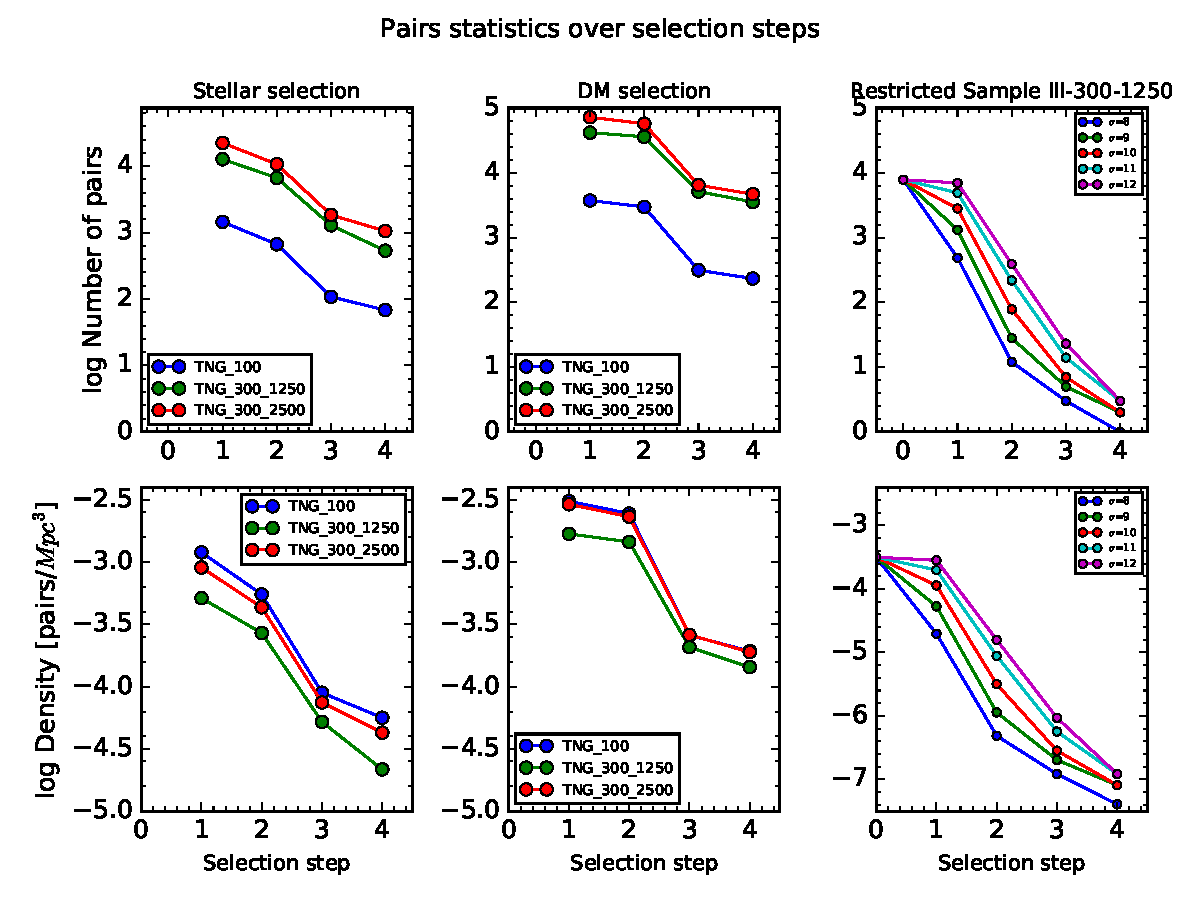
\includegraphics[scale=0.5]{NumberPairs.pdf}
\caption{\label{fig:pairs} Count of pairs (top row) and density defined as $[pairs/Mpc^3]$ at each selection step. In the left and center columns, stage \textit{0} corresponds to the original sample, and in the right column to the preliminary mass cut.}
\end{figure}
 
 
We calculated the average properties of the pair samples at each step and compare them between different simulations. The numbers in the x-axis correspond to the 4 constraints. The properties that are relative to a pair are reported after pair candidates have been selected, which means after applying the mass cut. 
 
\begin{figure*}
\centering
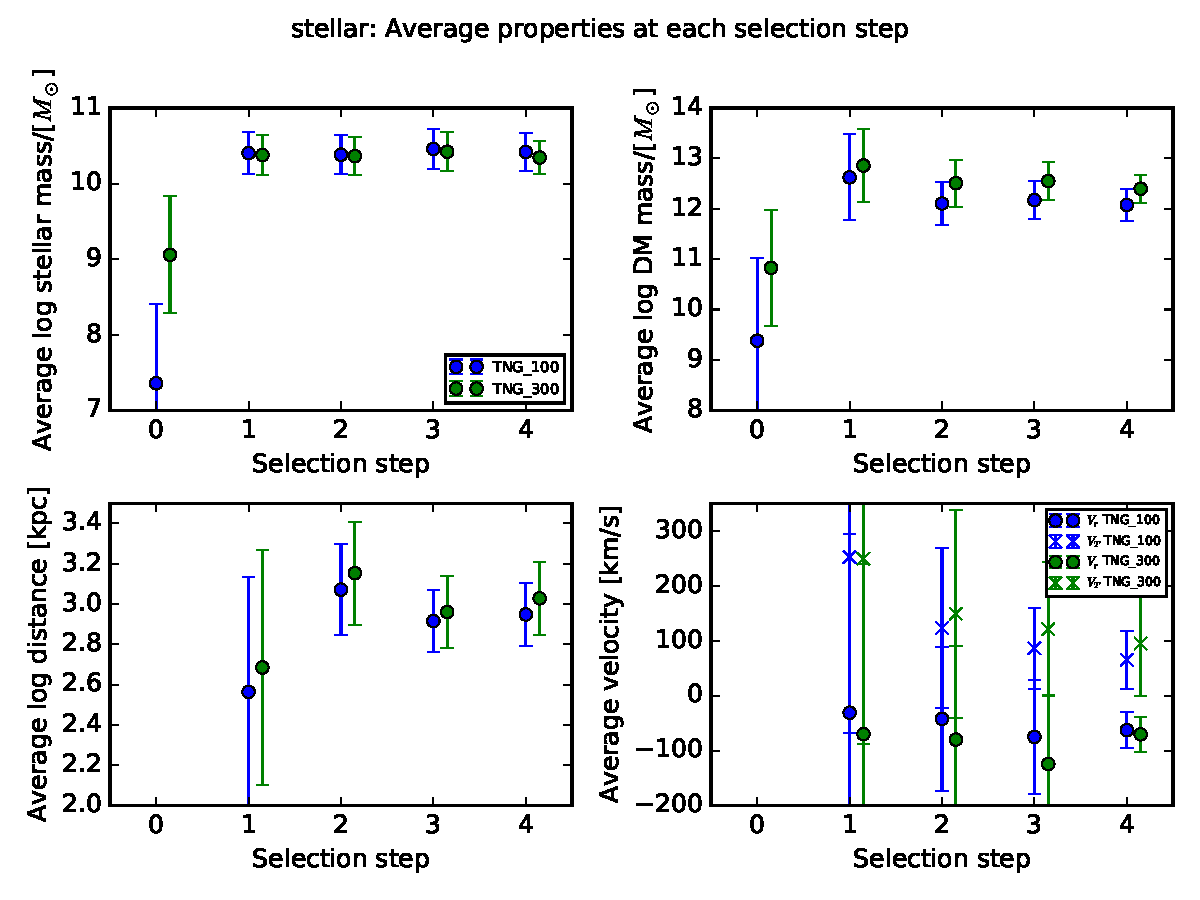
\includegraphics[scale=0.4]{avgProp/stellar_avgPropsTNG_100TNG_300.pdf}
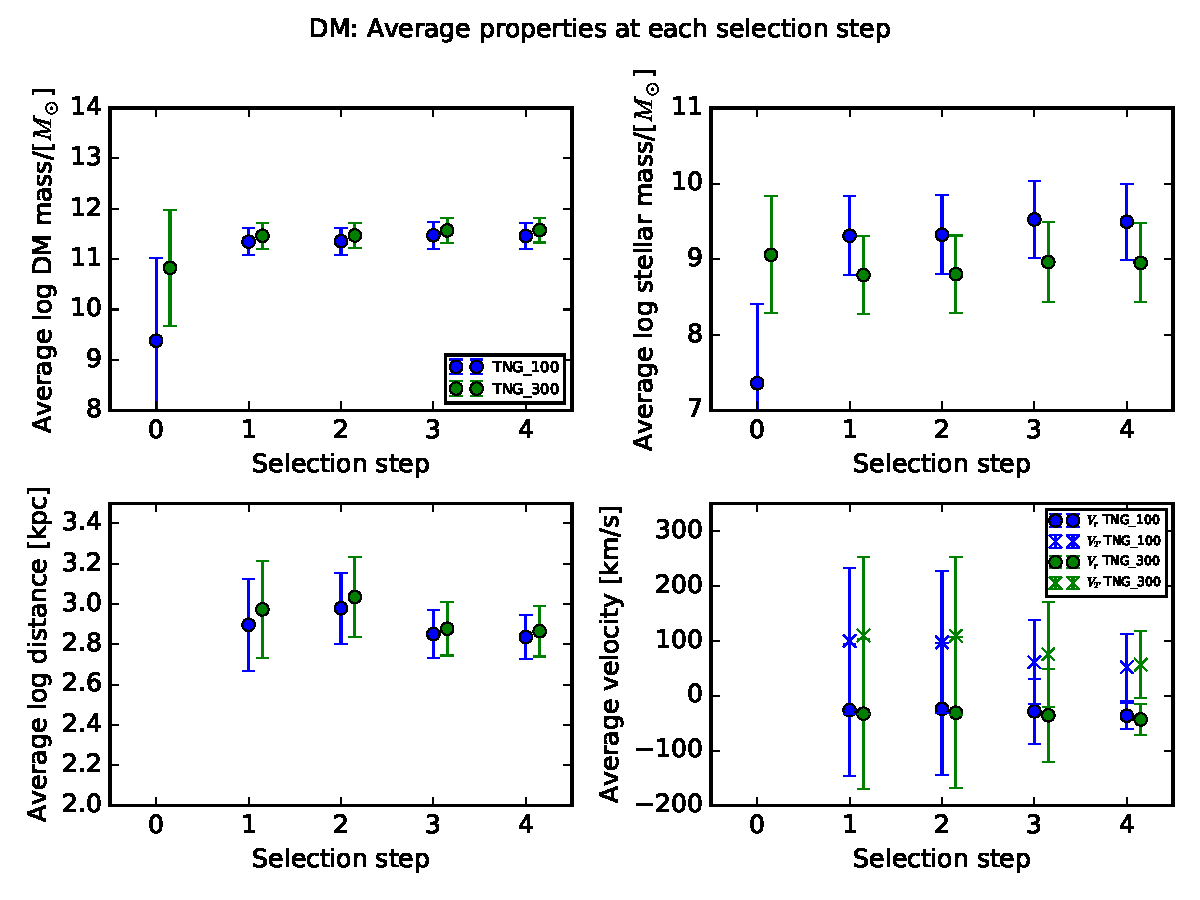
\includegraphics[scale=0.4]{avgProp/DM_avgPropsTNG_100TNG_300.pdf}
\caption{\label{fig:prop_100_300} Comparison between the average properties at each selection step for Illustris-100 and Illustris-300 (1820 and 1250 particles, respectively). Stage $0$ denotes the original sample.}
\end{figure*}

\begin{figure*}
\centering
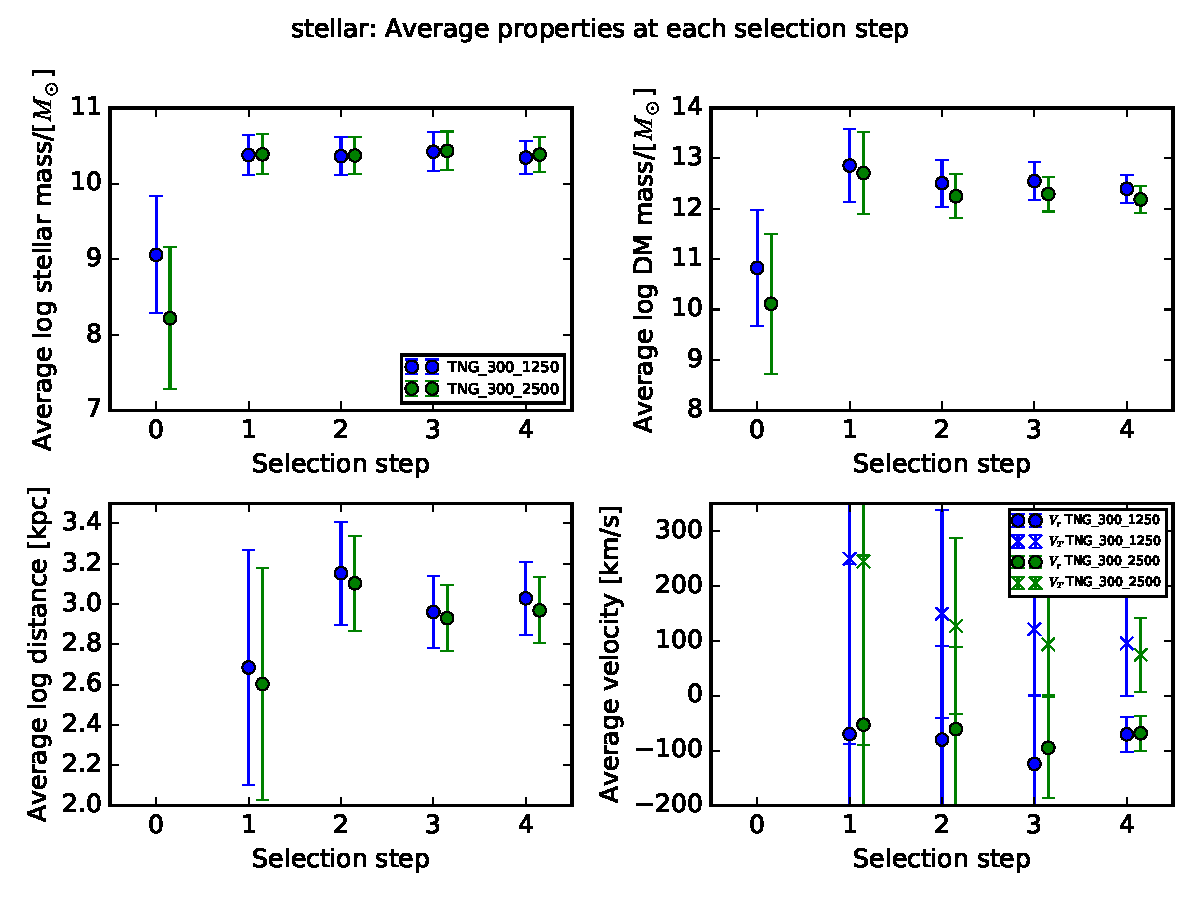
\includegraphics[scale=0.4]{avgProp/stellar_avgPropsTNG_300_1250TNG_300_2500}
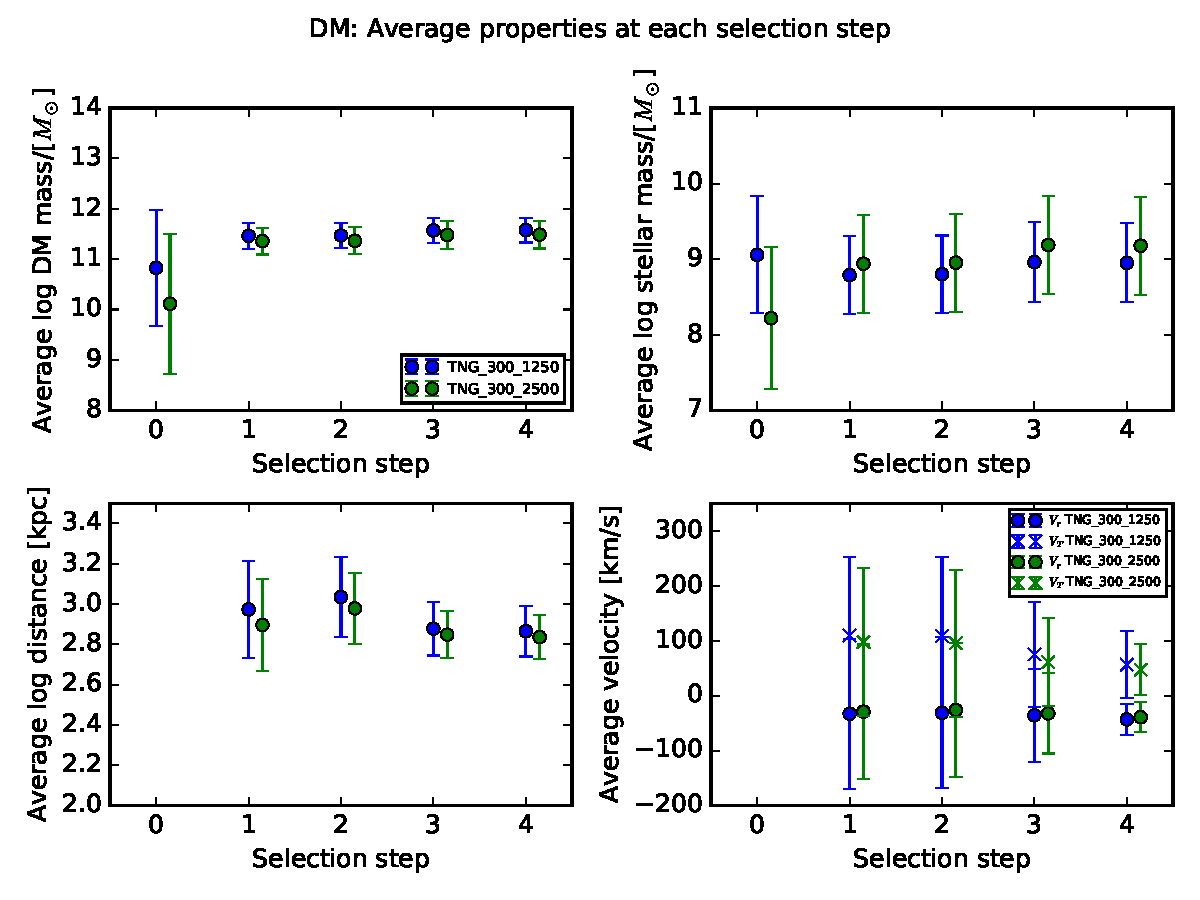
\includegraphics[scale=0.4]{avgProp/DM_avgPropsTNG_300_1250TNG_300_2500}
\caption{\label{fig:prop_300_300} .Comparison between the average properties over each selection step for Illustris-300 at two different resolutions (1250-2500 particles). Stage $0$ denotes the original sample.}
\end{figure*}

 


\bibliographystyle{mnras}
\bibliography{references}


\end{document}
